\begin{figure}
    \centering
    \begin{subfigure}[t]{0.3\textwidth}
        \centering
        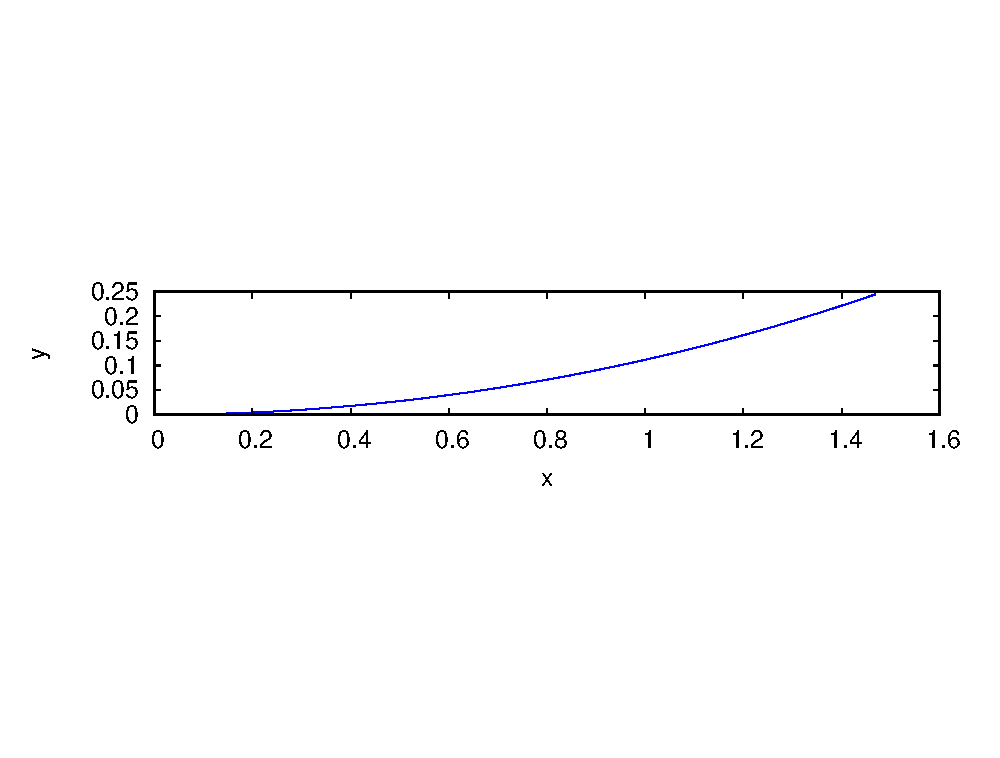
\includegraphics[width=\linewidth, height=30mm]{pic/_sol__1_0_1__0__10__1e2_trajectory}
        \caption{Траектория $X, Y$}
        \label{fig:_sol__1_0_1__0__10__1e2_trajectory}
    \end{subfigure}
    \begin{subfigure}[t]{0.3\textwidth}
        \centering
        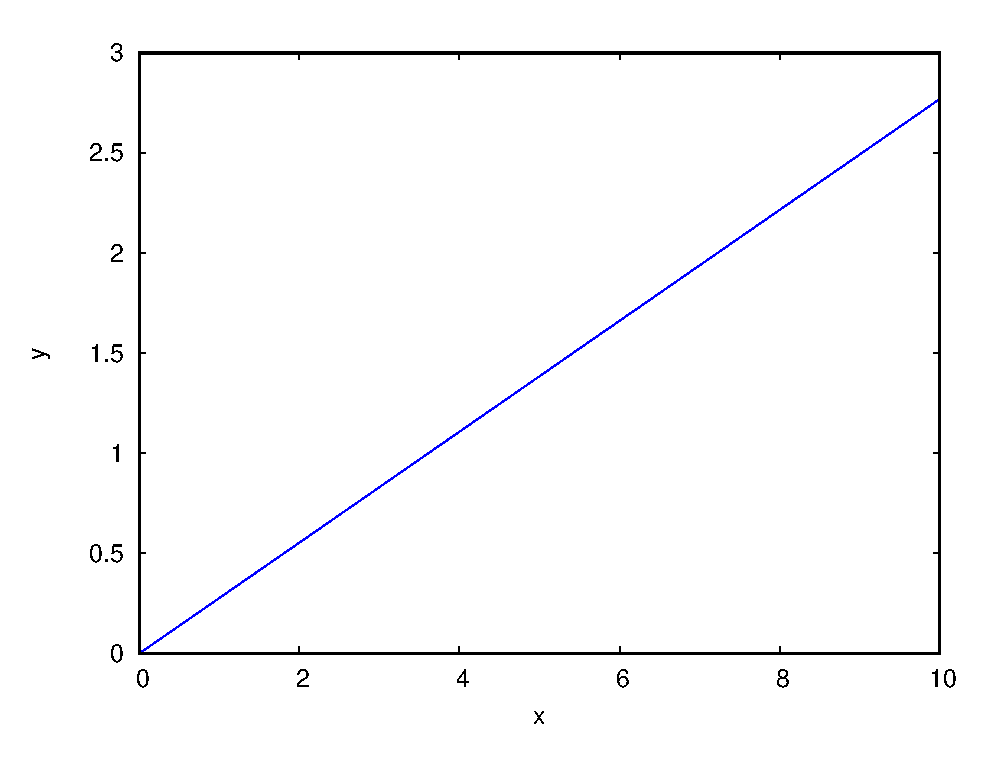
\includegraphics[width=\linewidth, height=30mm]{pic/_sol__1_0_1__0__10__1e2_theta}
        \caption{$\theta(t)$}
        \label{fig:_sol__1_0_1__0__10__1e2_theta}
    \end{subfigure}
    \vspace{12pt}
    
    \begin{subfigure}[t]{0.3\textwidth}
        \centering
        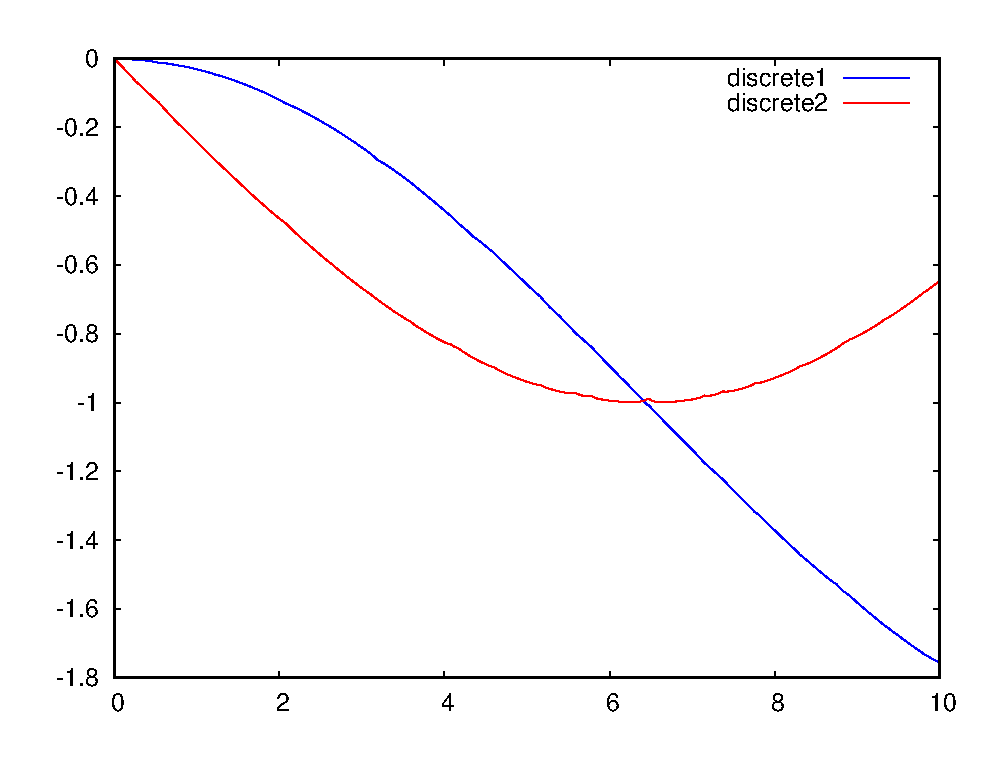
\includegraphics[width=\linewidth, height=30mm]{pic/_sol__1_0_1__0__10__1e2_nu12_centered}
        \caption{$\nu_1(t), \nu_2(t)$}
        \label{fig:_sol__1_0_1__0__10__1e2_nu12_centered}    
    \end{subfigure}
    \hfill
    \begin{subfigure}[t]{0.3\textwidth}
        \centering
        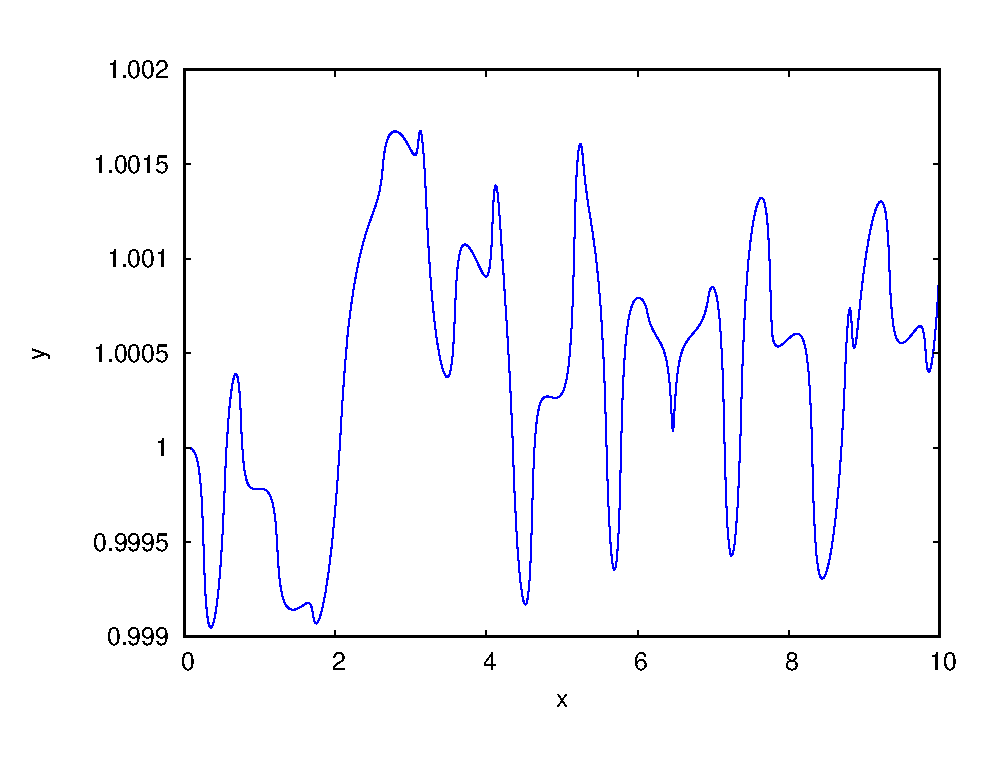
\includegraphics[width=\linewidth, height=30mm]{pic/_sol__1_0_1__0__10__1e2_nu3} \\
        \caption{$\nu_3(t)$}
        \label{fig:_sol__1_0_1__0__10__1e2_nu3}
    \end{subfigure}
    \hfill
    \begin{subfigure}[t]{0.3\textwidth}
        \centering
        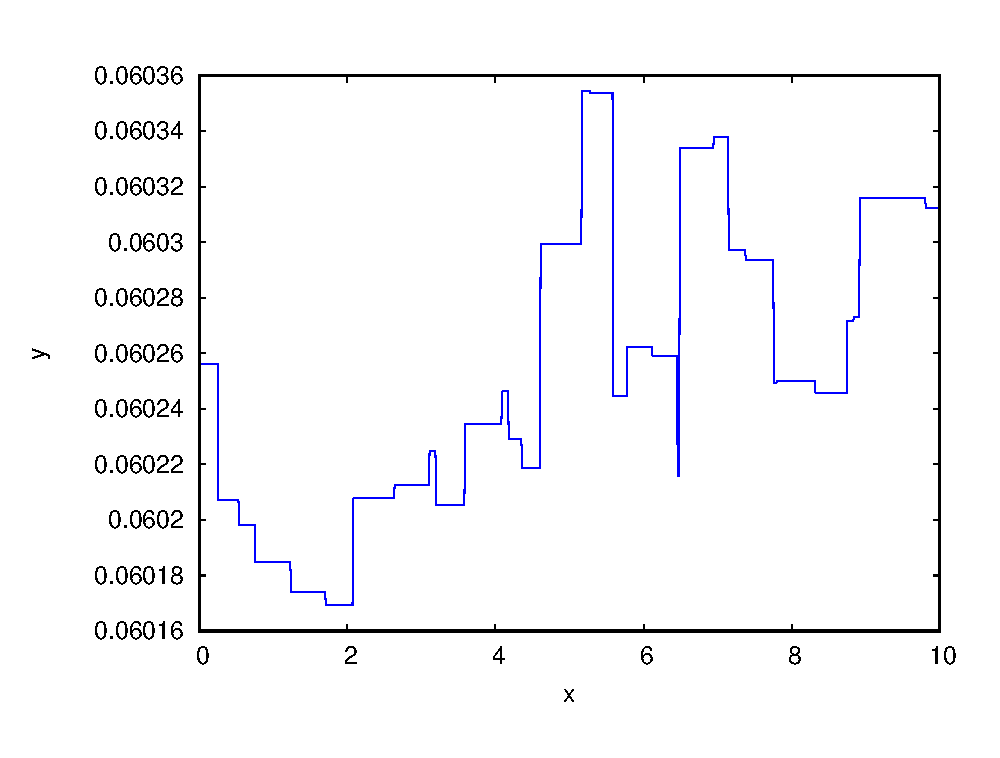
\includegraphics[width=\linewidth, height=30mm]{pic/_sol__1_0_1__0__10__1e2_kin_en}
        \caption{Кинетическая энергия}
        \label{fig:_sol__1_0_1__0__10__1e2_kin_en}
    \end{subfigure}
    
    \caption{Экипаж c роликами. Движение с закруткой ($\nu_1(0) = 1, \nu_2(0) = 0, \nu_3(0) = 1$) на коротком промежутке времени. Псевдоскорости не постоянны, виден ступенчатый вид кинетической энергии.}
    \label{fig:wrench_short}
\end{figure}
